\chapter{Software Architecture}
\label{chapter:architecture}

This chapter will discuss the software design behind this work.  It will cover the underlying tools, and then present the framework broken up into functional modules, rather than presenting the entire framework altogether.

\section{ROS}

I used ROS.  Look it up.

\section{ScaViSLAM ROS wrapper}

ScaViSLAM is standalone software that doesn't use any underlying frameworks such as ROS.  Therefore in order to use the ROS framework with ScaViSLAM, a ROS wrapper for ScaViSLAM needed to be developed.  The core functionality of scavislam was bundled into a library and contained within a package.

In order to do this, ScaViSLAM was split up into two packages; scavislam\_lib and scavislam\_ros.  All of the core functionality of ScaViSLAM was bundled into a library file and contained within the scavislam\_lib package.  To maintain minimal build dependencies and ensure fast compiling and linking, the scavislam\_lib has very minimal ROS code and therefore minimal ROS dependencies.  On the other hand, scavislam\_ros contains all of the neccessary ROS dependencies for visualization and control using standard ROS tools such as dynamic reconfigure and rviz.  This package acts as a bridge, converting scavislam datatypes to ROS datatypes. Fig. \ref{fig:scavislam_wrapper_dependencies} shows the ROS package dependencies for scavislam\_ros.  This clearly demonstrates the separation between ScaViSLAM dependencies and ROS dependencies.

This ROS wrapper allows complete replacement of the original ScaViSLAM GUI.  The ScaViSLAM graph may be visualized using rviz, and all visual tracking, keyframes and image pyramids may be visualized either in rviz or image\_view.  All of the original GUI functions may be manipulated using dynamic reconfigure.

\begin{figure}[h]
  \centering
    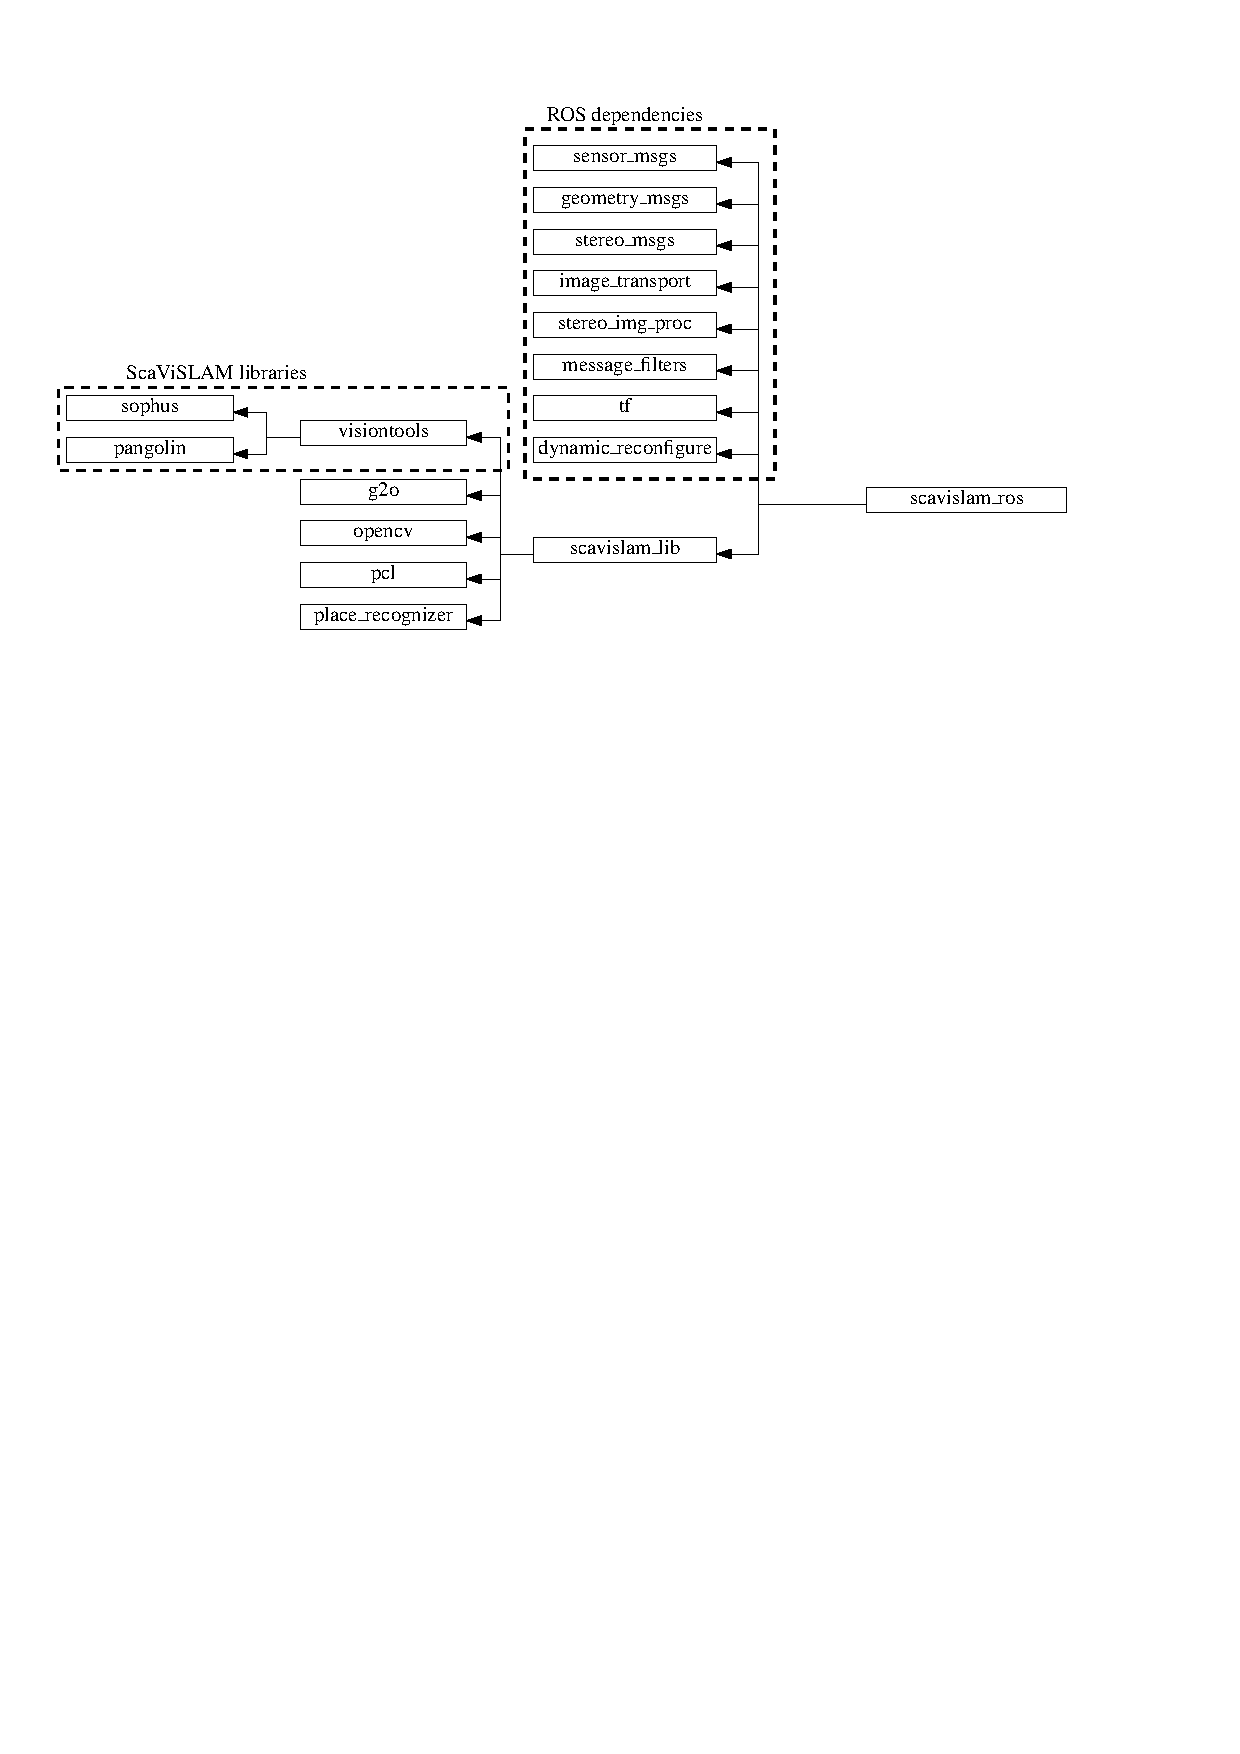
\includegraphics[width=1.0\textwidth]{chapters/images/ros_wrapper_dependencies}
  \caption{ROS package dependencies for the ScaViSLAM wrapper.  scavislam\_lib is designed to have minimal ros dependencies}
  \label{fig:scavislam_wrapper_dependencies}
\end{figure}


\section{Video input}

\begin{figure}[H]
  \centering
    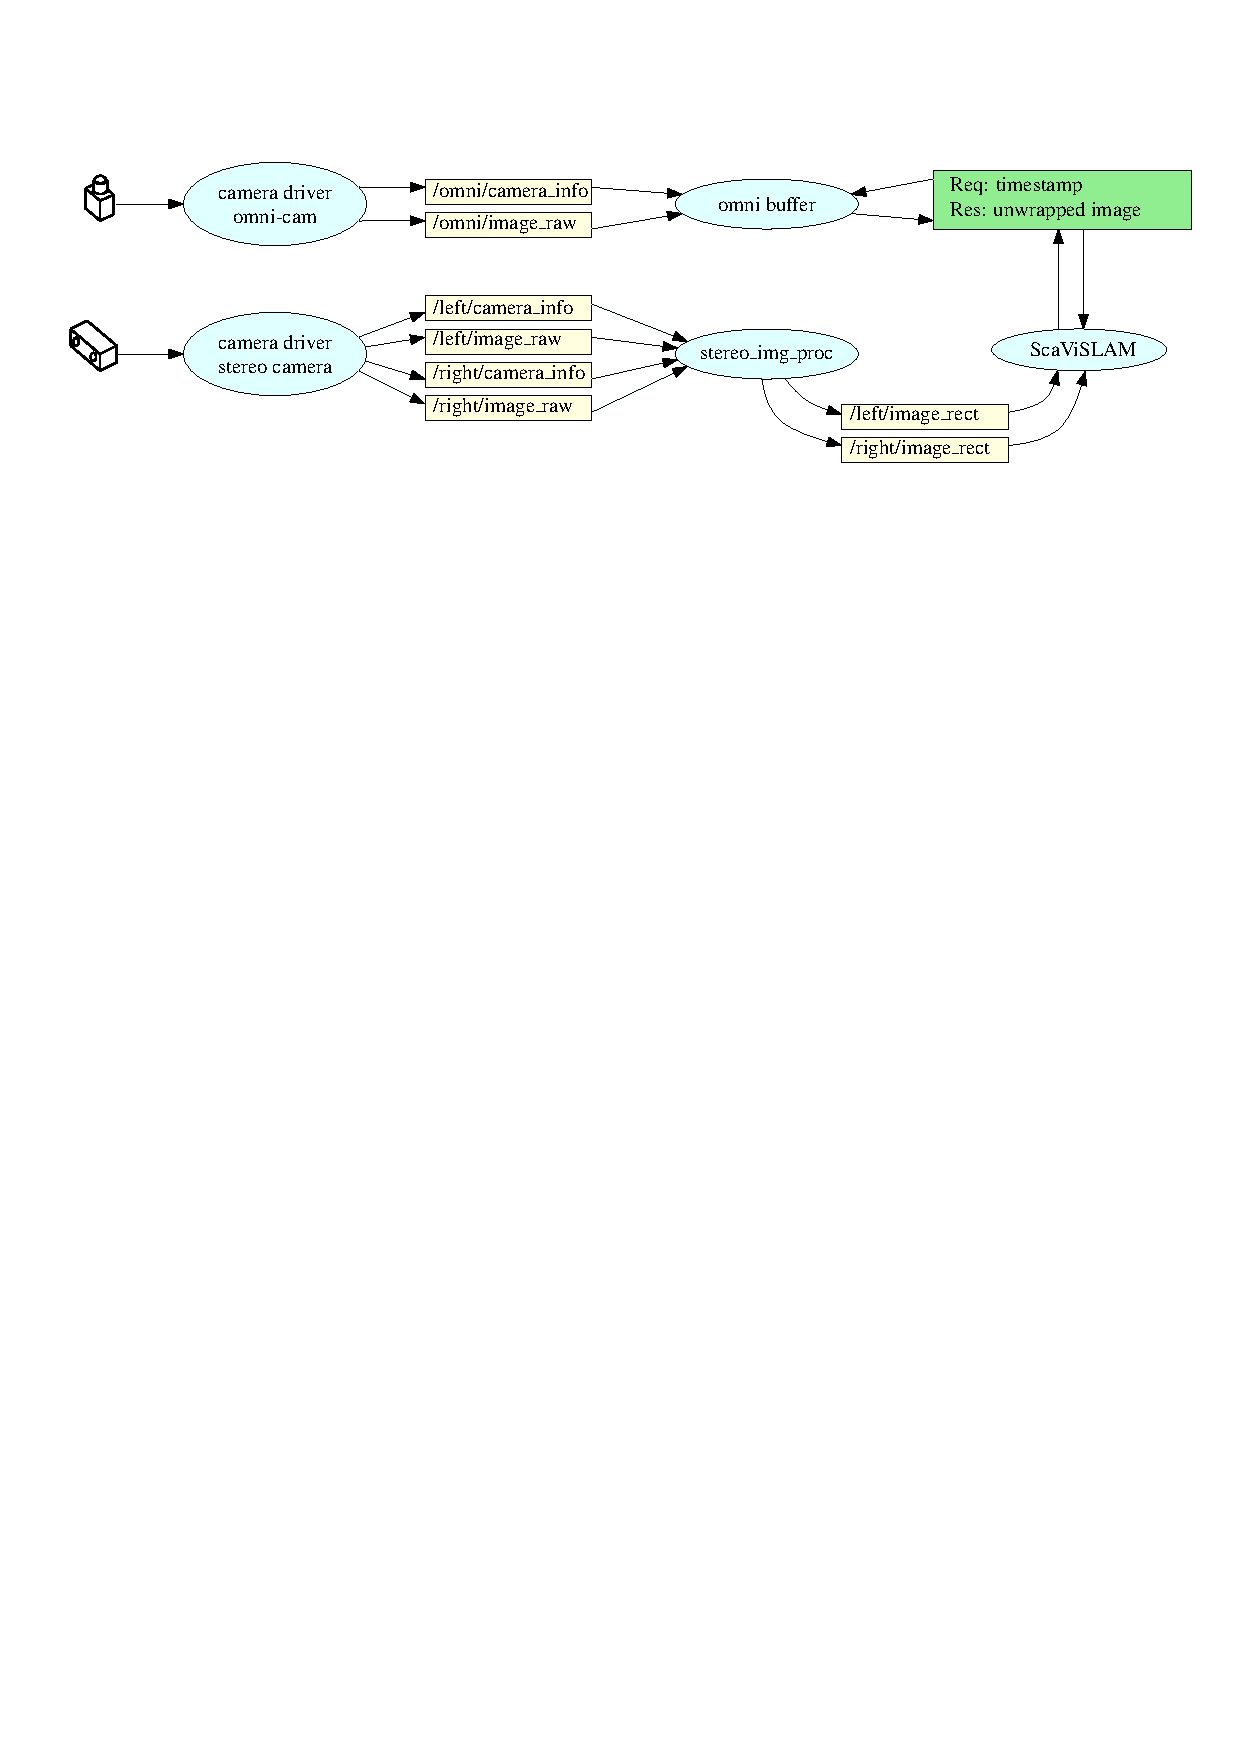
\includegraphics[width=1.1\textwidth]{chapters/images/input_architecture}
  \caption{System diagram for video input to ScaViSLAM system.  Blue are nodes, yellow topics and green services.}
  \label{fig:input_architecture}
\end{figure}

Fig. \ref{fig:input_architecture} outlines the system architecture for the input to ScaViSLAM.  For the stereo camera, a driver node receives data via Ethernet and publishes raw images and camera info.  The stereo image processing node subscribes to these topics, and accepts synchronized frames for processing.  Most importantly, it rectifies the images to non distorted images using the camera intrinsics supplied by camera info. (Sec. \ref{subsec:lense_distortion}) 

The pipeline for the omni camera images is significantly different to the stereo frames.  There are two main reasons for this, one being that there was no hardware synchronization available between omni camera and stereo used in this setup, which means that frames could not be accurately synchronized without potentially delaying stereo frames.  The second reason was to increase computational efficiency.  There is some computational load associated with unwrapping donut images to a spherical images.  The omni images are not required for every frame, they are only required for keyframes.  Therefore, only stereo frames which become keyframes require an associated omni camera image.

The omni camera driver receives donut images via firewire and publishes them.  The 'omni buffer' node subscribes to this topic and records every timestamped image to a buffer.  When ScaViSLAM creates a new keyframe, it then queries the omni buffer for an unwrapped image via a service call, providing the timestamp of the stereo frame as part of the request.  The omni buffer node searches through its buffer for the image closest to this timestamp, unwraps it, and returns it as a response to the service call.

This omni buffer node could be configured to unwrap and publish all omni camera frames, however the high resolution omni camera images at 30hz makes processing every frame very computationally expensive.

The ROS tool dynamic reconfigure can be used to configure the camera drivers.  This allows adjusting of gain/shutter controls, resolution, image depth etc.

\section{Image based place recognition}

\begin{figure}[h]
  \centering
    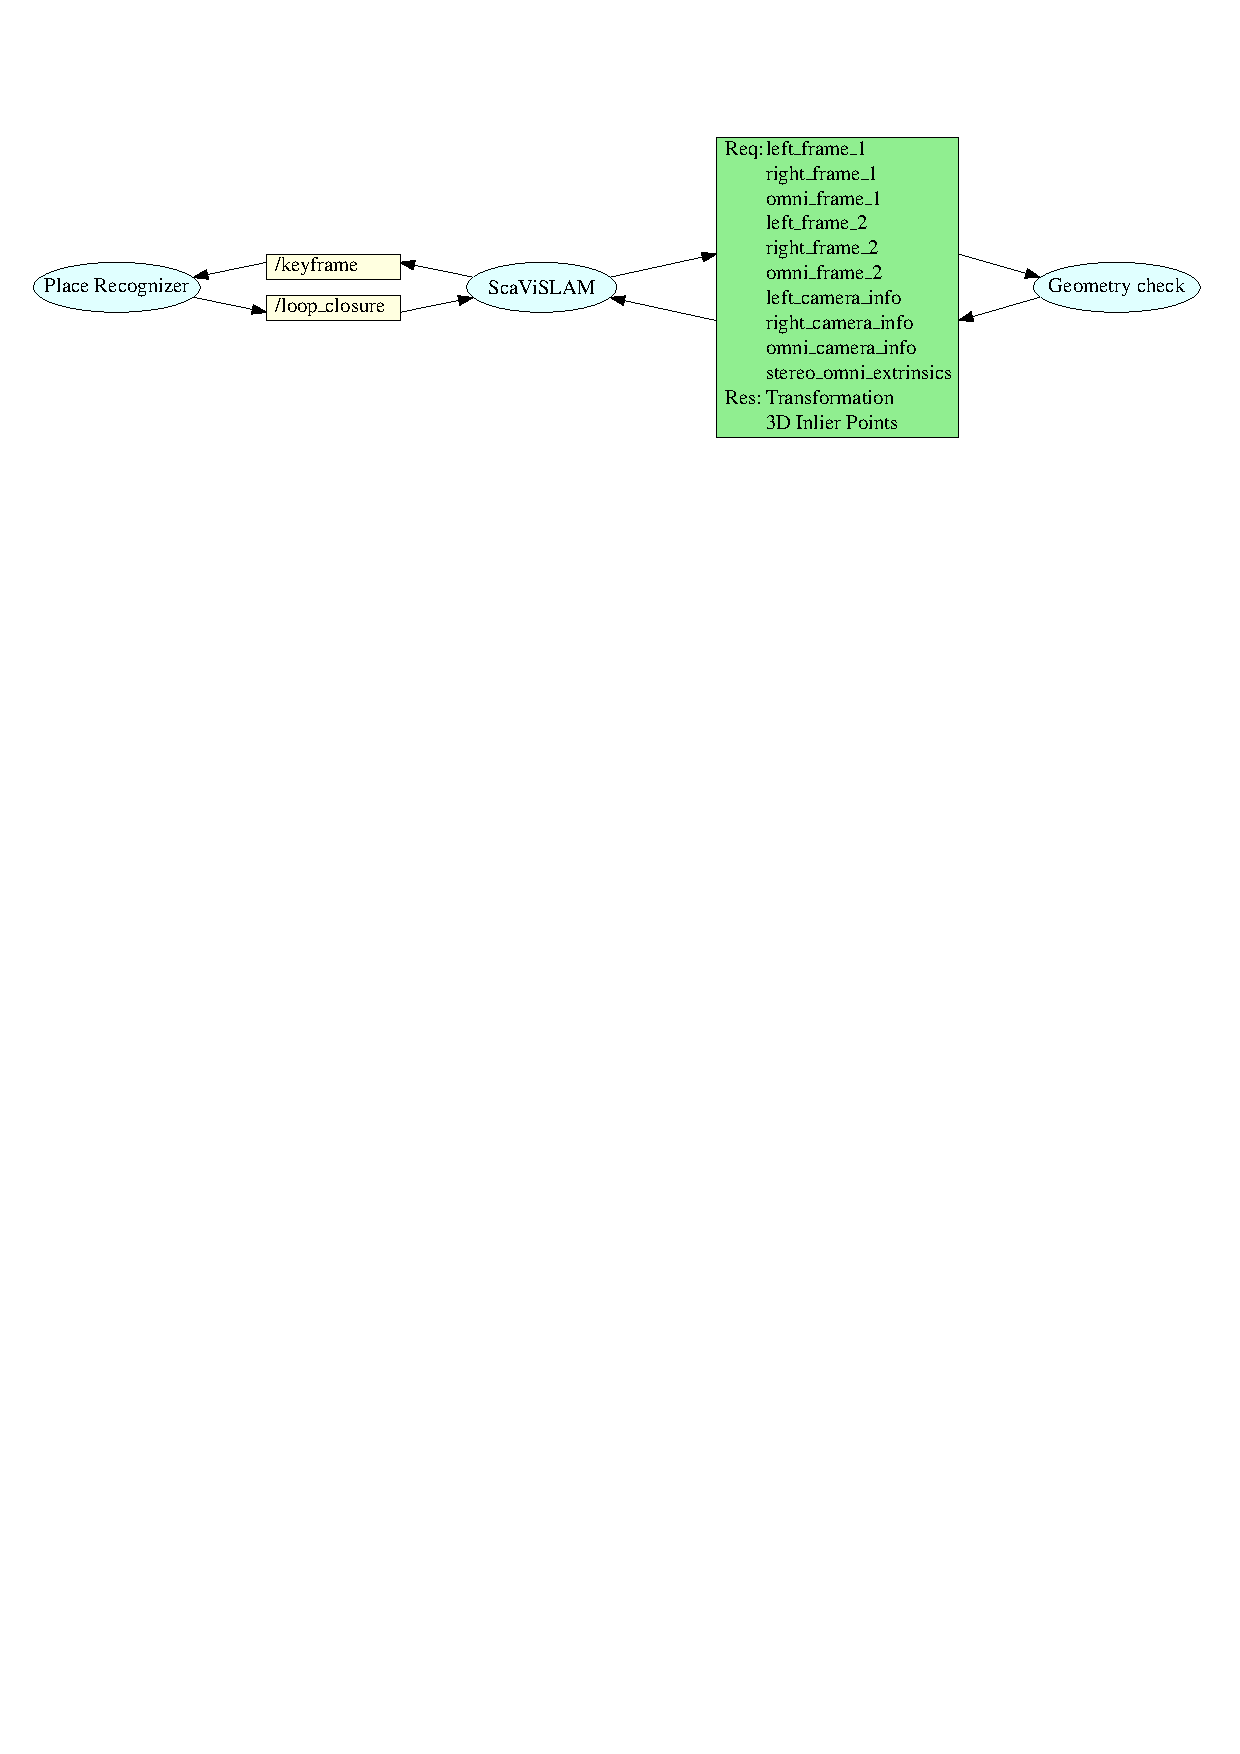
\includegraphics[width=1.1\textwidth]{chapters/images/loop_close_architecture}
  \caption{System diagram for image based loop closure for ScaViSLAM.  Blue are nodes, yellow topics and green services.}
  \label{fig:loop_close_architecture}
\end{figure}

The place recognition and geometry check pipeline were both moved into separate nodes from ScaViSLAM, and a successful loop closure involves communication with both.  The motivation for separating the place recognizer node is obvious as it has very clearly defined input and outputs.  Input is a keyframe image and associated id (/keyframe in Fig \ref{fig:loop_close_architecture}), and output is a pair of ids for a successful match (/loop\_closure in Fig \ref{fig:loop_close_architecture}).  This separation allows easy replacement or modification of the place recognizer implementation without impacting any other code.  It also allows the place recognizer to run in a separate thread.

Although the input/output requirements of the geometry check node are not as simple as that of the place recognizer, there are still a number of reasons to separate it into a different node.  First of all it provides a clear separation between ScaViSLAM code and the omni-loop-closure code to be developed.  Secondly, by taking only images as an input, and being agnostic of keyframe ids and keyframe storage, this geometry check can easily be used by other SLAM systems to perform geometry checks.  The service call shown in Fig \ref{fig:loop_close_architecture} is for an omni-loop-closure.  However the geometry check node also supports stereo pair or mono pair pair geometry checks.  

Finally this architecture allows easy changing between the omni-loop-closure version and the original ScaViSLAM system, which is a requirement for evaluation.  ScaViSLAM only needs to call the stereo pair service instead of the omni-loop-closure service for the original system.

The overall flow for a loop closure is as follows.  ScaViSLAM publishes keyframes as they are created.  The place recognizer encodes a keyframe to the bag of words representation as described in Section \ref{sec:bag_of_words} and associates this new representation with the keyframe id.  The original image is then discarded by the place recognizer.  For every new keyframe the place recognizer searches for matches.  One or more results may then be returned by the place recognizer, in the form of publishing 'potential' loop closure messages, where a single message contains just the two matching ids.  ScaViSLAM subscribes to this potential loop closure topic, and for every id pair, will obtain all the relevant images from the keyframe storage and then make a geometry check service call.  If the geometry check is successful, then the new SE(3) edge as returned from the geometry check will be added to the SLAM graph.

\section{Visualization and Control}

\begin{figure}[h]
  \centering
    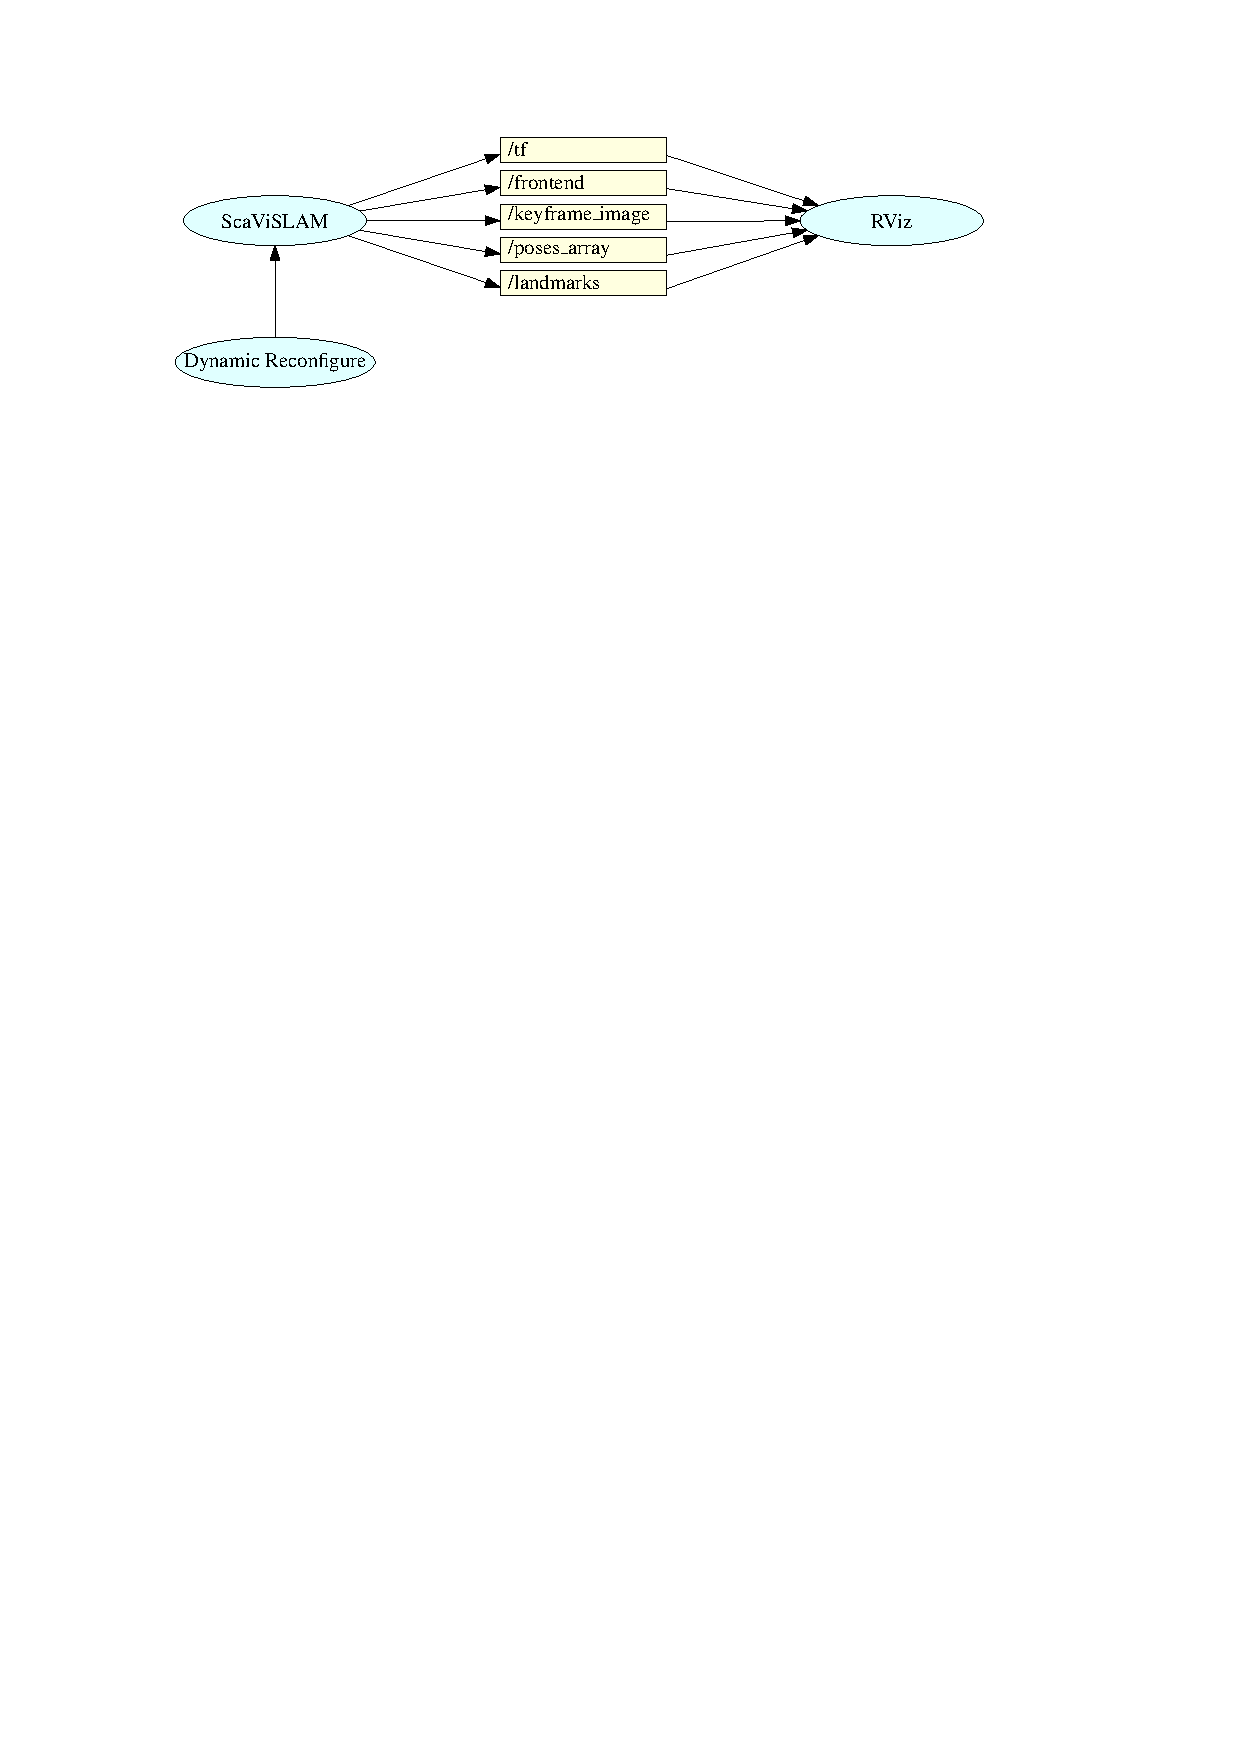
\includegraphics[width=1.0\textwidth]{chapters/images/visualization_architecture}
  \caption{System diagram for vizualization and user input.}
  \label{fig:visualization_architecture}
\end{figure}

Fig. \ref{fig:visualization_architecture} depicts the system architecture for visualization and control of ScaViSLAM.  Topics /frontend and /keyframe\_image are image topics.  The /frontend topic shows the visual tracking against the current keyframe and keyframe\_image allows the user to select and show various keyframes using dynamic reconfigure.  These can both show different image pyramid levels of their respective images also using dynamic reconfigure.

The topics /poses\_array and /landmarks are to visualize the SLAM graph.  The keyframes are visualized by /poses\_array and landmarks within the current inner window are published to /landmarks.  In addition, the current keyframe and current pose with respect to the current keyframe are published to /tf.  This allows easy comparison with groundtruth data as well as debugging of transforms using RViz.

Control of runtime parameters and visualization options is achieved through dynamic reconfigure.  The actual mechanism of this control is a number of topics and services auto generated by the dynamic reconfigure package.  This is not visualized here as there would be a large number of topics and services which would clutter the diagram.

